%
% $RCSfile: reflection.tex,v $
%
% Copyright (c) 2004. Christian Heller. All rights reserved.
%
% No copying, altering, distribution or any other actions concerning this
% document, except after explicit permission by the author!
% At some later point in time, this document is planned to be put under
% the GNU FDL license. For now, _everything_ is _restricted_ by the author.
%
% http://www.cybop.net
% - Cybernetics Oriented Programming -
%
% http://www.resmedicinae.org
% - Information in Medicine -
%
% @author Christian Heller <christian.heller@tuxtax.de>
%

\paragraph{Reflection}
\label{reflection_heading}

The \emph{Reflection} pattern \cite{buschmann} (also known under the synonyms
\emph{Open Implementation} or \emph{Meta-Level Architecture}) provides a
mechanism to change the structure and behaviour of a software system
\emph{dynamically}, that is at runtime, which is why that mechanism is sometimes
called \emph{Run Time Type Identification} (RTTI). A reflective system owns
information about itself and uses these to remain changeable and extensible.

\begin{figure}[ht]
    \begin{center}
        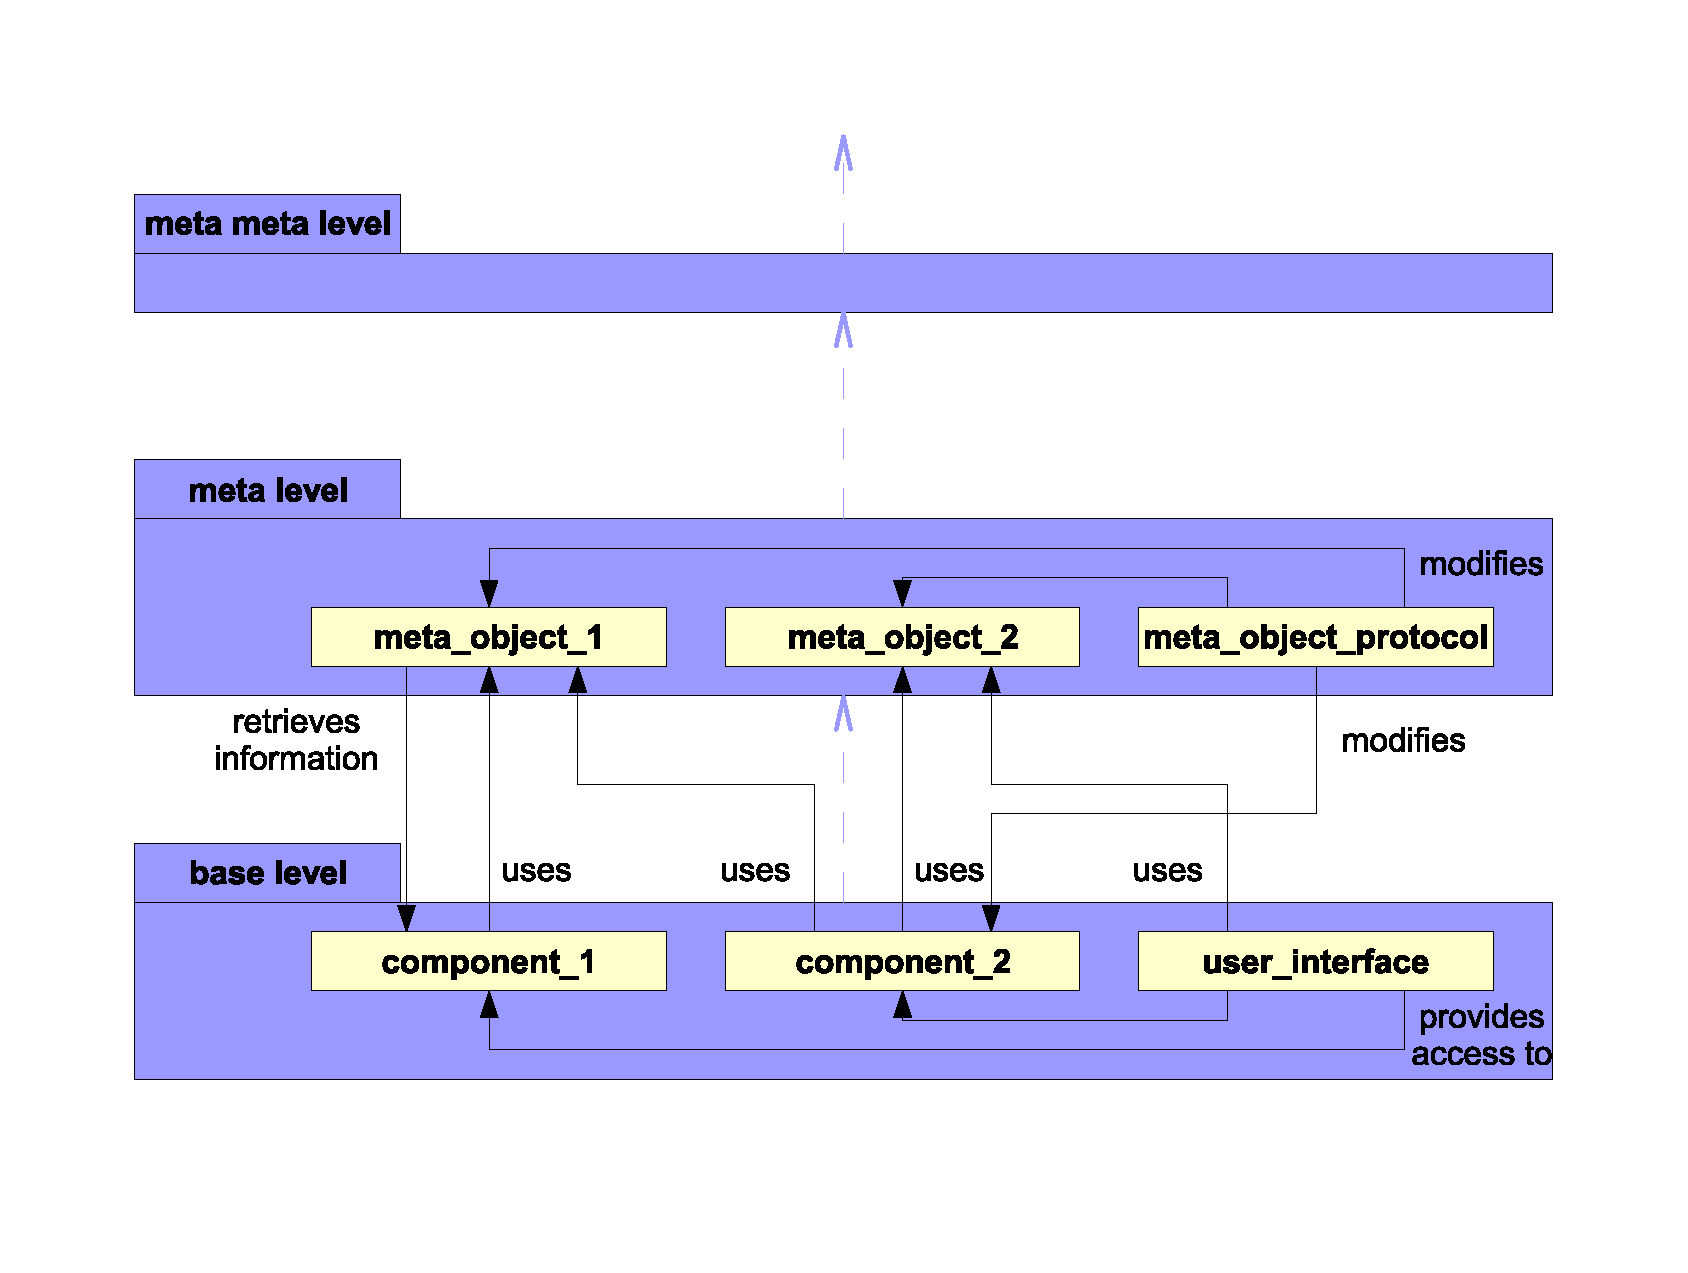
\includegraphics[scale=0.3]{vector/reflection.eps}
        \caption{Reflection Pattern}
        \label{reflection_figure}
    \end{center}
\end{figure}

Reflective information \emph{about} something is called \emph{Meta Information}.
Therefore, the level above the \emph{Base Level} in figure \ref{reflection_figure}
is labelled \emph{Meta Level}. The base level depends on the meta level, so that
changes in the meta level will also affect the base level. All manipulation of
meta objects happens through an interface called \emph{Meta Object Protocol}
(MOP), which is responsible for checking the correctness of- and for performing
a change. If a further level holds information about the meta level, then that
additional level is called \emph{Meta Meta Level}, and so forth.

Many examples of meta level architectures exist. In his book
\emph{Analysis Patterns} \cite{fowler1997}, Fowler uses them extensively.
He talks of \emph{Knowledge Level} (instead of meta level) and
\emph{Operational Level} (instead of base level). Elements of the
\emph{Unified Modeling Language} (UML) are defined in an own meta model
\cite{uml}. And the principles of reflection are also supported by several
programming languages, such as \emph{Smalltalk} \cite{smalltalk} and
\emph{Java} \cite{java}.

Classes (types) in a system have a static structure, as defined by the developer
at design time. Normally, most classes belong to the base level containing the
application logic. As written before, one way to change the structure and
behaviour of classes at runtime is to introduce a meta level providing type
information, in other words functionality that \emph{all} application classes
need. This helps avoid redundant implementations of the same functionality.

Looking closer at functionality, it turns out that some basic features like
persistence and communication occur repeatedly in almost all systems, while
other parts are specific to one concrete application. Traditionally, the
application classes in the base level have to cope with general system
functionality although that is not in their original interest. It therefore
seems logical to try to divide application- and system functionality, and to put
the latter into a meta level.
